\section{Аналитическая часть}

В этом разделе будет представлен анализ существующих способов представления объектов, алгоритмов построения реалистического изображения, текстурирования и моделей освещения.

\subsection{Описание трёхмерного объекта}

В компьютерной графике существует множество способов представления объектов. В данной работе необходимо выделить такие способы, которые позволяет показать объём модели и наложить текстуру. В связи с этими требованиями можно рассмотреть следующие варианты:

\begin{itemize}[leftmargin=1.6\parindent]
	\item[---] геометрические примитивы;
	\item[---] воксельная модели;
	\item[---] полигональные модели.
\end{itemize}

\subsubsection{Геометрические примитивы}

Примитив может быть описан некоторой функцией, принимающей параметры, например, центр и радиус для сферы или ширину, высоту и глубину для параллелепипеда. В качестве таких примитивов могут выступать любые геометрические объекты: куб, конус, пирамида, сфера или цилиндр.

Достоинства:
\begin{itemize}[leftmargin=1.6\parindent]
	\item[---] простота построения изображения модели;
	\item[---] малое количество информации для хранения представления. объекта.
\end{itemize}

Недостатки:
\begin{itemize}
	\item[---] сложность создания реалистичной моделей из геометрических примитивов;
	\item[---] трудность наложения текстур.
\end{itemize}

\subsubsection{Воксельная модель}

Двумерные модели можно описать с помощью пикселей. Аналогично можно и описывать трёхмерные модели из вокселей, маленьких кубиков. Они являются элементами объёмного изображения, содержащие значения элементов растра в трёхмерном виде.

Достоинства:
\begin{itemize}
	\item[---] хорошо подходит для моделирования непрерывных сред;
	\item[---] хорошо подходит для трассировки.
\end{itemize}

Недостатки:
\begin{itemize}
	\item[---] большой расход памяти;
	\item[---] низкое разрешение.
\end{itemize}

\subsubsection{Полигональная модель}

Полигональная модель использует полигональную сетку, которая является совокупностью связанных между собой выпуклых многоугольников (полигонов), аппроксимирующих поверхность модели. Представление модели в виде многоугольников упрощает их рендер. Чаще всего как полигон используются треугольник, так как он является простейшим многоугольником и все остальные многоугольники могут быть разбиты на треугольники.\cite{data_view}

Данным способом можно описать объекты любой формы с хорошим разрешением и детализацией. Детализация зависит от количества полигонов в сетке. Время рендера напрямую зависит от количества полигонов в модели.

Благодаря тому что полигоны это плоские многоугольники их легко использовать для имитации неровностей, изменяя их нормали, и текстурирования, заранее указав текстурные координаты.

Достоинства:
\begin{itemize}
	\item[---] широко используются в компьютерной графике;
	\item[---] необходимо вычислять только координаты вершин при преобразованиях;
\end{itemize}

Недостатки:
\begin{itemize}
	\item[---] сложные алгоритмы визуализации;
	\item[---] аппроксимация приводит к погрешностям.
\end{itemize}

\subsubsection{Вывод}

После анализа вышеописанных вариантов в качестве способа представления объектов сцены была выбрана полигональная модель. Так как в отличии от других вариантов с помощью полигональной сетки можно представить объекты любой формы в хорошем разрешении и большой детализацией, используя относительно небольшой объём памяти для хранения.

\subsection{Алгоритм построения трёхмерного изображения}

В этом разделе будут рассмотрены алгоритмы построения трёхмерного изображения, которые будут использоваться в написанном ПО. Эти алгоритмы являются важнейшей частью всей программы и выполняют основную работу по рендеру результирующего изображения.

\subsubsection{Алгоритм с Z-буфером}

Алгоритм работает в пространстве изображения и в нём используется 2 буфера: Z-буфер(буфер глубины) и буфер кадра, размер соответствуют количеству пикселей на экране. В Z-буфере находится информация о координате z для каждого пикселя, а в буфере кадра его интенсивность. В начале работы буферы заполняются минимальным значением координаты z и интенсивностью фона соответственно. Затем каждый многоугольник преобразуется в растровую форму и записывается в буфер кадра, при этом не производится никакого начального упорядоченивания.

\begin{figure}[hbtp]
	\centering
	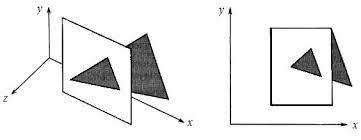
\includegraphics[scale=0.6]{img/zbuf.jpg}
	\caption{Пример работы алгоритма с использованием Z-буфера}
\end{figure}

В процессе работы глубина каждого нового пикселя сравнивается с глубиной, занесённой в буфер глубины. Если глубина нового пикселя меньше, то в буфер кадра заносится данные интенсивности нового пикселя, а в z-буфер новую координату z. Если же глубина нового пикселя больше, то данные в буферах не меняются.

Достоинствами данного алгоритма является простота его реализации и отсутствие сортировки элементов сцены. К недостаткам же можно отнести большой объём используемой памяти и трудоемкость реализации эффектов прозрачности и преломления, а также устранения ступенчатости.

\subsubsection{Алгоритм с обратной трассировкой лучей}

Является модификацией простого алгоритма трассировки лучей и отличается лишь тем что лучи испускается из камеры, а не из источников света.

Сам алгоритм работает по следующему принципу: из камеры выпускается луч, который называется первичным, и ищется пересечения луча с каким-либо объектом сцены. Если пересечение не находится, то результатом является фоновая интенсивность, иначе проверяется освещенность точки пересечения первичного луча и объекта сцены всеми источниками света. Для это пускается теневой луч в направлении каждого источника света. Если он пересекает какой-либо объект, то источник света не видим из точки пересечения, то есть объект находится в тени относительного этого источника и соответственно он не освещает данную точку. Если же теневой луч не встретил никаких объектов на своём пути, то интенсивность рассчитывается в соответствии с моделью освещения. Результатом являет суммарная интенсивность от всех видимых источников света.\cite{alg}

Если тела обладает отражающими свойства, то просчитывается и испускается отражённый луч, для которого рекурсивно выполняются те же операции как и для первично. Аналогично программа работает с преломлёнными лучами.

Достоинства данного алгоритма является высокий реализм получаемого изображения, учёт таких физических явлений как тень, преломление, отражение. Также алгоритм легко поддаётся распараллеливанию.

Основным недостатком является производительность. Каждый раз необходимо просчитывать множество новых лучей, что создаёт немалую нагрузку на вычислительные устройства.

\subsubsection{Вывод}

Для создания реалистичного изображения лучше всего подходит алгоритм трассировки лучей, так как он даёт наиболее приближенный к реальности результат и учитывает отражения, прозрачность и тени. Основным недостатком является его производительность. Алгоритм с использованием Z-буфера же можно использовать для предпросмотра сцены где может потребоваться рендер в реальном времени, которые трудно реализуем алгоритмом трассировкой лучей без соответствующего графического ускорителя.

\subsection{Алгоритмы наложения текстур на трёхмерные объекты}

\subsubsection{Афинное текстурирование}

Самый дешевый способ интерполяции между тремя текстурными координатами треугольника — использовать линейную интерполяцию с барицентрическими координатами. Введём координаты текстуры $u$, $v$. Они указывают на определённый пиксель текстуры, тексель. Для вершит полигонов изначально заданы текстурные координаты, указываю на соответствующий тексель. Чтоб не высчитывать значения $u$ и $v$ для каждого пикселя проекции полигона, можно воспользоваться билинейной интерполяцией, используя уже известные координаты тексилей вершин треугольника. Основным недостатком этого метода является игнорирование координаты $z$, из-за чего текстура может искажаться и выглядить нереалистично.

\subsubsection{Перспективно-корректное текстурирование}

Искажения в афинном текстурировании вызваны допущением что $u$, $v$ изменяются по экрану линейно. Это не так. Точные значения координат тексилей можно считать по точечным формулам, но это не эффективно. Проще воспользоваться фактом что $u/z$ и $v/z$ линейно зависят от координат проекции треугольника. Достаточно посчитать для каждой вершины $1/z$, $u/z$ и $v/z$, а затем их линейно интерполировать по всему полигону. Сами же точные значения $u$ и $v$ считаются как: \[ u=(u/z)/(1/z) \] \[ v=(v/z)/(1/z) \]

\subsubsection{Вывод}

Наиболее реалистичным методом является перспективно-корректное текстурирование, так как в его основе лежит точное текстурирование, учитывающее перспективу в отличии от афинного метода.

\subsection{Модель освещения трёхмерных объектов}

\subsubsection{Модель Ламберта}

Простейшая модель освещения, чисто диффузное освещение. Считается, что свет падающий в точку, одинакового рассеивается по всем направлением полупространства. Таким образом, освещенность в точке определяется только плотностью света в точке поверхности, а она линейно зависит от косинуса угла падения. Считается по формуле:
\[
I = k_{d}(\vec{n}, \vec{l}),
\]
где:
\begin{itemize}
	\item[---] $k_{d}$ - коэффицент диффузного отражения;
	\item[---] $\vec{n}$ -  нормаль;
	\item[---] $\vec{l}$ - еденичные вектор, напрвленный к источнику света.
\end{itemize}

\subsubsection{Модель Фонга}

Модель расчёта освещения трёхмерных объектов, в том числе полигональных моделей и примитивов, а также метод интерполяции освещения по всему объекту. Это локальная модель освещения, то есть она учитывает только свойства заданной точки и источников освещения, игнорируя эффекты рассеивания, линзирования, отражения от соседних тел. Эта модель состоит из диффузной составляющей и зеркальной. Благодаря зеркальной составляющей на объектах появляеюся блики. Интенсивность в точке зависит от того насколько близки отражённый вектор к вектору направленному из точки падения в сторону наблюдетеля. В модели учитывается интенсивность фонового, диффузного и зеркально освещёния. Для расчёта диффузной составляющей используется модель Ламберта.\cite{light}

Считается по формуле:
\[
I = k_{a}I_{a} + k_{d}(\vec{n}, \vec{l}) + k_{s}(\vec{n}, \vec{r})^n,
\]
где:
\begin{itemize}
	\item[---] $k_{d}$ - коэффицент диффузного отражения;
	\item[---] $k_{s}$ - коэффицент зеракльного отражения;
	\item[---] $k_{a}$ - коэффицент рассеянного отражения;
	\item[---] $I_{s}$ - интенсивность фонового освещения;
	\item[---] $\vec{n}$ -  нормаль;
	\item[---] $\vec{l}$ - еденичные вектор, напрвленный к источнику света;
	\item[---] $\vec{l}$ - еденичные вектор, напрвленный к наблюдателю;
	\item[---] $n$ - степень, аппроксимирующая пространственное распределение зеркально отраженного света.
\end{itemize}

\subsubsection{Модель Уиттеда}

Модель освещенности Уиттеда является одной из самых распространенных и наиболее часто используемой моделью в методе трассировки лучей. Использует для расчёта интенсивности глобальную модель освещения, учитывающую свет провзаимодействовавший с другими объектами. Помимо учёта фоновой, диффузной и зеркальной компонент в этой модели ещё учитывается интенсивность отражённого и преломлённого света от других тел. Согласно этой модели суммарная интенсивность определяется следующим уравнением:

\begin{equation}
	I = k_{a}I_{a}C + k_{d}I_{d}C + k_{s}I_{s} + k_{r}I_{r} + k_{t}I_{t},
	\label{eq:whitted_general}
\end{equation}
где 
\begin{itemize}
	\item[---] $k_{a}$ - коэффициент рассеянного отражения;
	\item[---] $k_{d}$ - коэффициент диффузного отражения;
	\item[---] $k_{s}$ - коэффициент зеркального отражения;
	\item[---] $k_{r}$ - коэффициент отражения;
	\item[---] $k_{t}$ - коэффициент преломления;
	\item[---] $I_{a}$ - интенсивность фонового компоненты;
	\item[---] $I_{d}$ - интенсивность диффузной компонеты;
	\item[---] $I_{s}$ - интенсивность зеркального компоненты;
	\item[---] $I_{r}$ - интенсивность отражённого луча;
	\item[---] $I_{t}$ - интенсивность преломлённого луча;
	\item[---] $C$ - цвет.
\end{itemize}

\subsubsection{Вывод}

Для получения наиболее реалистических изображений была выбрана модель Уиттеда как самая подходящая и реалистичная, так как она учитывает такие эффекты, как отражение, прозрачность, преломление, тень.

\pagebreak